\tikzstyle{block} = [draw, rectangle, text width=2cm, text centered, minimum height=1.2cm, node distance=2.7cm]
\tikzstyle{computation-block} = [block, fill=blue!30]
\tikzstyle{memory-block} = [block, fill=green!30]
\tikzstyle{cache-block} = [block, fill=orange!30]

\begin{center}
	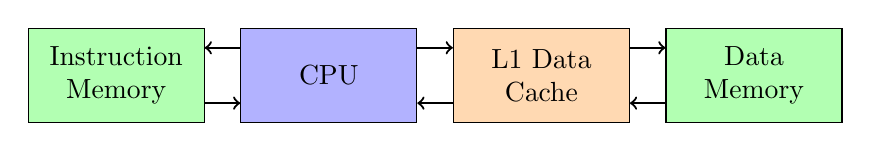
\begin{tikzpicture}
	
	 \node [computation-block] (CPU) {CPU};
	 \node [memory-block, left of=CPU] (Imem) {Instruction Memory};
	 \node [cache-block, right of=CPU] (DCache) {L1 Data Cache};
	 \node [memory-block, right of=DCache] (Dmem) {Data Memory};
	
	\draw [thick] [->] ([yshift=1em]DCache.east)-- ([yshift=1em]Dmem.west);
	\draw [thick] [<-] ([yshift=-1em]DCache.east)-- ([yshift=-1em]Dmem.west);

	\draw [thick] [->] ([yshift=1em]CPU.east)-- ([yshift=1em]DCache.west);
	\draw [thick] [<-] ([yshift=-1em]CPU.east)-- ([yshift=-1em]DCache.west);
	
	\draw [thick] [->] ([yshift=1em]CPU.west)-- ([yshift=1em]Imem.east);
	\draw [thick] [<-] ([yshift=-1em]CPU.west)-- ([yshift=-1em]Imem.east);
	
	\end{tikzpicture}
\end{center}